\section{Criterion}

\begin{frame}{Why a new criterion?}

  For STM performance,
  \begin{itemize}
  \item invisible reads = no contention for read-only transactions
  \item disjoint-access parallelism = disjoint transactions do not contend
  \end{itemize}
  \input{slides/figures/motivation}
  \begin{itemize}
  \item but $h_3 \notin \OPA$ ... ($\tOne$ cannot know that $\tThree \hb \tTwo$).
  \item \underline{usual solution}: use global clock to commit updates
  \end{itemize}
\end{frame}

\begin{frame}{The synchronization wall}

  \begin{figure}
    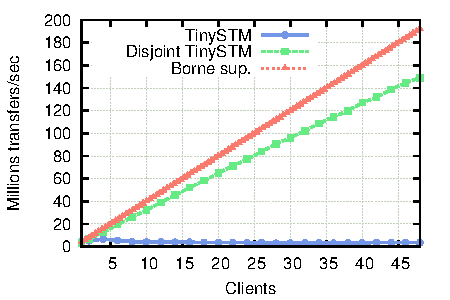
\includegraphics{results/bank-motiv.pdf}
  \end{figure}
  Bank benchmark (transferts between accounts) \\
  Disjoint TinySTM = distinct runtimes \\
  \hspace{8.6em}     + threads access disjoint accounts
\end{frame}

\begin{frame}{Stricter serializability (\SPSER)}

  \begin{definition}[Binding]
    $T_i$ bounds to $T_j$ when $r_i(x_j)$ and $T_i$ concurrent to $T_j$
  \end{definition}

  \pause
  \smallskip
  
  \begin{definition}[Fair binding]
    When for every $y_k$ read by $T_i$ before $x_j$, $T_j \depends T_k$ holds or $T_k$ commits after $T_j$.
  \end{definition}

  \pause
  \smallskip

  \begin{definition}[Stricter serializability]
    $h \in \SPSER$ when $h \in \SSER$ and $T_i \in \aborted{h}$ implies either 
    (i) $T_i$ observes a strictly consistent snapshot in $h$, or (ii) one of its bindings is unfair.
  \end{definition}
  
\end{frame}

\begin{frame}{For which applications?}

  Application state:
  \begin{itemize}
  \item References = pointer between objects
  \item Object graph = objects + references
  \end{itemize}

  \bigskip

  The transactions ($\mathcal{T}$) ensure that:
  \begin{itemize}
  \item the object graph always forms a tree, and
  \item each transaction traverses the tree via a simple top-down path.
  \end{itemize}

  \bigskip
  
  \begin{theorem*}
    Let $H_{\mathcal{T}}$ be the histories of the set of transactions $\mathcal{T}$.\\
    The relation $(\SPSER \inter H_{\mathcal{T}} \setminus \RCAD) \subset \OPA$ is true.\footnotemark
  \end{theorem*}

  \footnotetext{
    $h \in \RCAD = (r_i(x_k), w_i(y_i) \in h \land x_k \ll_h x_j) \implies c_i \hb_{h} c_j$
  }

\end{frame}

\begin{frame}{For which applications?}
  
  \begin{theorem*}
    Let $H_{\mathcal{T}}$ be the histories of the set of transactions $\mathcal{T}$.\\
    The relation $(\SPSER \inter H_{\mathcal{T}} \setminus \RCAD) \subset \OPA$ is true.
  \end{theorem*}

  \bigskip
  [proof sketch]

  \begin{columns}
    \begin{column}{0.3\textwidth}
      \begin{figure}[!h]
        \centering
        \fontsize{8}{11}\selectfont
        \begin{tikzpicture}[scale=0.8]          
          \node[] at (0,0) (8) {8};
          \node[] at (-1,-1) (3) {3};
          \node[] at (-2,-2) (1) {1};
          \node[] at (0,-2) (6) {6};
          \node[] at (-1,-3) (4) {4};
          \path[] (8) edge (3);
          \path[] (3) edge (6);
          \path[] (3) edge (1);
          \path[] (6) edge (4);
        \end{tikzpicture}        
      \end{figure}
      ${\color{OliveGreen}{T_1}}=contains(6)$
    \end{column}
    %
    \begin{column}{0.3\textwidth}
      \begin{figure}[!h]
        \centering
        \fontsize{8}{11}\selectfont
        \begin{tikzpicture}[scale=0.8]
          \node[] at (0,0) (8) {8};
          \node[] at (-1,-1) (3) {3};
          \node[color=gray] at (-2,-2) (1) {1};
          \node[] at (0,-2) (6) {6};
          \node[] at (-1,-3) (4) {4};
          \path[] (8) edge (3);
          \path[] (3) edge (6);
          \path[,color=gray] (3) edge (1);
          \path[] (6) edge (4);
        \end{tikzpicture}
      \end{figure}
      ${\color{red}{T_2}}=del(1)$
    \end{column}
    %
    \begin{column}{0.3\textwidth}
      \begin{figure}[!h]
        \centering
        \fontsize{8}{11}\selectfont
        \begin{tikzpicture}[scale=0.8]          
          \node[] at (0,0) (8) {8};
          \node[] at (-1,-1) (3) {3};
          \node[] at (-2,-2) (1) {1};
          \node[] at (0,-2) (6) {6};
          \node[] at (-1,-3) (4) {4};
          \path[] (8) edge (3);
          \path[] (3) edge (6);
          \path[] (3) edge (1);
          \path[] (6) edge (4);
          \node[] at (1,-3) (7) {\textbf{7}};
          \path[,thick] (6) edge (7);
        \end{tikzpicture}
      \end{figure}
      ${\color{blue}{T_3}}=add(7)$
    \end{column}
  \end{columns}
  
\end{frame}

\begin{frame}{For which applications?}

  \begin{columns}
    \begin{column}{0.6\textwidth}
      \begin{itemize}
      \item[] Assume $\tThree$ bound to $\tOne$
      \item[] (Case $T_? \hb \tOne$)
      \item[] \hspace{1em} $\tOne \depends T_?$ (simple path property)
      \item[] (Otherwise.)
      \item[] \hspace{1em} $h \notin \RCAD \implies c_? \hb {\color{blue}{c_3}}$
      \item[] $\Rightarrow$ Binding $r_1({\color{blue}{6}})$ is \underline{fair}.
      \end{itemize}      
    \end{column}
    %
    \begin{column}{0.3\textwidth}
      \begin{figure}[!h]
        \centering
        \fontsize{8}{11}\selectfont
        \begin{tikzpicture}[scale=0.8]          
          \node[] at (0,0) (8) {8};
          \node[] at (-1,-1) (3) {?};
          \node[color=blue] at (0,-2) (6) {6};
          \node[] at (-1,-3) (4) {4};
          \path[] (8) edge (3);
          \path[] (3) edge (6);
          \path[] (6) edge (4);
          \node[] at (1,-3) (7) {7};
          \path[] (6) edge (7);
        \end{tikzpicture}
      \end{figure}
      ${\color{OliveGreen}{T_1}}=r_1(8).r_1(?).r_1({\color{blue}{6}})$\\
      \bigskip
      ${\color{OliveGreen}{T_1}}=contains(6)$ \\
      ${\color{red}{T_2}}=del(1)$ \\
      ${\color{blue}{T_3}}=add(7)$
    \end{column}
  \end{columns}
  
\end{frame}


